% \begin{abstract}
% A computationally-fast inverse design method for nanophotonic structures is presented. The method is based on two complementary convex optimization problems which modify the dielectric structure and resonant field respectively. The design of one- and two-dimensional nanophotonic resonators is demonstrated and is shown to require minimal computational resources.
% \end{abstract}
% 
% \begin{thebibliography}{99}
% \bibitem{Yee66} K. Yee, ``Numerical solution of initial boundary value problems involving Maxwell’s equations in isotropic media,'' IEEE Trans. Antennas Propag. Mag. \textbf{14}, 302-307 (1966).
% \bibitem{AB74} M.~Albani and P.~Bernardi, ``A Numerical Method Based on the Discretization of Maxwell Equations in Integral Form,'' IEEE Trans.~Microwave Theory Tech. \textbf{22}, 446-450 (1974).
% \bibitem{GA79} J.~M.~Gerardy and M.~Ausloos, ``Absorption spectrum of clusters of spheres from the general solution of Maxwell's equations. The long-wavelength limit,'' Phys.~Rev.~B \textbf{22}, 4950-4959 (1979).
% \bibitem{Lon09} P. Deotare, M. McCutcheon, I. Frank, M. Khan, M. Loncar, ``High quality factor photonic crystal nanobeam cavities,'' Appl. Phys. Lett. \textbf{94}, 121106 (2009).
% \bibitem{Sch02} J. Vuckovic, M. Loncar, H. Mabuchi, A. Scherer, ``Design of photonic crystal microcavities for cavity QED,'' Phys. Rev. E \textbf{65}, 1-11 (2002).
% \bibitem{Nod05} Y.~Akahane, T.~Asano, B.~Song, S.~Noda, ``Fine-tuned high-Q photonic-crystal nanocavity,'' Opt. Express \textbf{13}, 1202-1214 (2005).
% \bibitem{Lip08} A. Gondarenko, M. Lipson, ``Low modal volume dipole-like dielectric slab resonator,'' Opt. Express \textbf{16}, 17689-17694 (2008).
% \bibitem{SD05} A. Hakansson, J. Sanchez-Dehesa, ``Inverse designed photonic crystal de-multiplex waveguide coupler,'' Opt. Express \textbf{13}, 5440-5449 (2005).
% \bibitem{Sig04} P. Borel, A. Harpøth, L. Frandsen, M. Kristensen, P. Shi, J. Jensen, and O. Sigmund, ``Topology optimization and fabrication of photonic crystal structures,'' Opt. Express \textbf{12}, 1996-2001 (2004).
% \bibitem{Vuc05} D. Englund, I. Fushman, and J. Vuckovic. ``General Recipe for Designing Photonic Crystal Cavities,'' Opt. Express \textbf{12}, 5961–5975 (2005).
% \bibitem{cholmod} \emph{CHOLMOD} software package, accessed via \emph{Matlab}.
% \bibitem{mycomp} Intel Core 2 Quad $2.5$GHz, 8Gb RAM.
% \bibitem{JJ99} S.~G.~Johnson, J.~D.~Joannopoulos, ``Block-iterative frequency-domain methods for Maxwell’s equations in a planewave basis,'' Opt.~Express \textbf{8}, 967-970 (1999).
% \bibitem{BV04} S. Boyd, L. Vandenberghe, \emph{Convex Optimization} (Cambridge University Press, 2004).
% \bibitem{CVX} M. Grant and S. Boyd, \emph{CVX: Matlab software for disciplined convex programming}, \texttt{http://stanford.edu/$\sim$boyd/cvx}, June 2009.
% \bibitem{Hen06} K. Hennessy, C.~Högerle, E.~Hu, A. Badolato, A. Imamoğlu, ``Tuning photonic nanocavities by atomic force microscope nano-oxidation,'' Appl.~Phys.~Lett.~\textbf{89}, 041118 (2006).
% \bibitem{Aka05} B.~-S.~Song, S.~Noda, T.~Asano, Y.~Akahane, ``Ultra-high-Q photonic double-heterostructure nanocavity,'' Nat. Mater. \textbf{4}, 207-210 (2005).
% \bibitem{Riv09} K.~Rivoire, Z.~Lin, F.~Hatami, W.~Ted Masselink, and J.~Vuckovic, ``Second harmonic generation in gallium phosphide photonic crystal nanocavities with ultralow continuous wave pump power,'' Optics Express \textbf{17}, 22609-22615 (2009).
% \end{thebibliography}
% 
\chapter{Direct design}
\section{Introduction}
Numerous numerical methods have been devised to solve Maxwell's equations in both time\cite{Yee66} and frequency\cite{AB74,GA79} domains. We refer to these schemes as direct solvers, since they compute the electric and magnetic fields based on current sources, charge distributions and surrounding dielectric and/or metallic structures. While extremely useful in simulating optical components, using direct methods to design optical components, especially in two or three dimensions,  typically requires an extremely time-consuming direct search in a large parameter space\cite{Lon09,Sch02,Nod05,Lip08,SD05}.

On the other hand, an inverse solver would be much more adept in such design and optimization problems\cite{Sig04,Vuc05}. In this work, we define the inverse problem as that where the electromagnetic field is known, but the surrounding structure is not known. The goal in the inverse problem is, then, to find a dielectric structure that will produce that specific electromagnetic field profile.

We show that one can design nanophotonic resonators by specifying the electromagnetic field and its desirable characteristics (such as cavity quality (Q) factor and/or mode volume) and then using an inverse solver to find the corresponding dielectric structure. We show that the inverse method used is not only computationally-fast, but is also able to optimize for multiple device characteristics and produce multiple resonances, both of which are very difficult using direct methods. 

\section{Numerical Setup}
We start from the time-harmonic eigenvalue equation 
\begin{equation}
\nabla \times \epsilon^{-1} \nabla \times H = \left(\frac{\omega}{c}\right)^2 H
\label{trad ev}\end{equation}
where $H$, $\epsilon$, $\omega$ and $c$ are the magnetic field, relative permittivity, resonance frequency and speed of light respectively. To solve the problem numerically, $H$ and $\epsilon$ are discretized in space using the standard Yee cell used in finite difference methods\cite{Yee66}. Also, the curl operators, since they are linear, are represented by the matrix $A$. Eq.~\eqref{trad ev} can now be written as 
\begin{equation}
A Y A x = \xi x
\label{lin ev}\end{equation}
where
\begin{align*}
&A \text{ is the discretized curl operator,} \\
&Y = \text{diag}(\epsilon^{-1}) \text{ is the diagonal matrix representing the dielectric structure,} \\
&x \text{ is a vector representing $H$, and} \\
&\xi =  \left(\frac{\omega}{c}\right)^2. 
\end{align*}
In this form, given $Y$, we can solve the direct problem by computing $x$ using an eigenvalue solver\cite{JJ99}. However, we note that eq.~\eqref{lin ev} is also linear in $Y$, which allows us, if $x$ is held constant, to solve the inverse problem by expressing eq.~\eqref{trad ev} as
\begin{equation}
By = d
\label{inv ls}\end{equation}
where
\begin{align*}
&B = A \cdot \text{diag}(Ax), \\
&d = \xi x\text{, and} \\
&y = 
\begin{bmatrix}
\epsilon_1^{-1} \\ \epsilon_2^{-1} \\ \vdots
\end{bmatrix} \text{ the variable for which we solve.}
\end{align*}
Here, $\text{diag}(Ax)$ is the matrix with the values of $Ax$ along the main diagonal and zeros elsewhere.

\section{Least-Squares Method in 1D}
\subsection{Least-Squares}
\begin{figure}[htbp]\centering
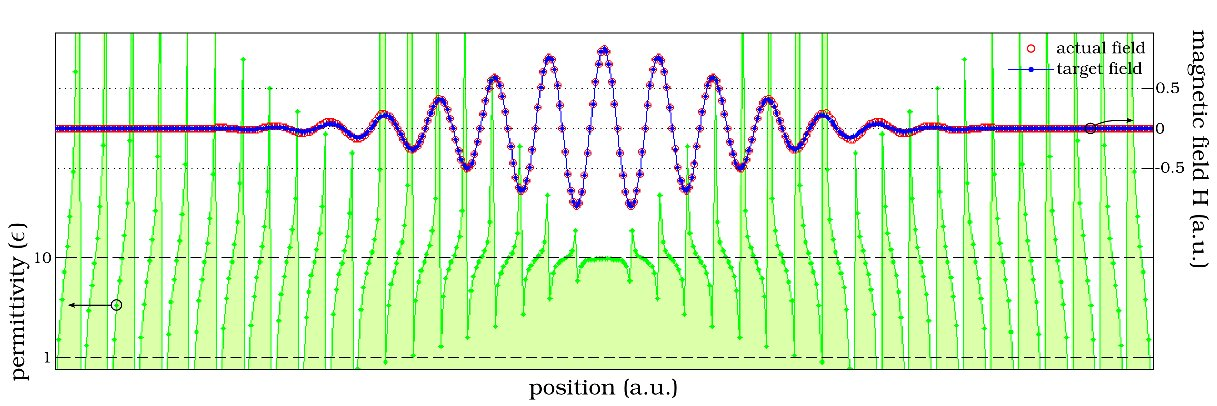
\includegraphics[width=\textwidth]{p1/leastsquares}
\caption{Inverse design of a one-dimensional structure using the unmodified least-squares method. The target field is a sinusoid within a Gaussian envelope. The computed dielectric structure (green area) supports a field (red circles) that exactly matches the target field (blue line). The entire design process is also extremely fast and takes less than $1$ second to complete on a generic desktop computer~\cite{mycomp}. The periodic singularities in the dielectric structure are non-physical and will be addressed later in the article.}
\label{ls pic}\end{figure}
The result of applying this method to a simple one-dimensional problem is shown in Fig.~\ref{ls pic}. A generic least-squares solver~\cite{cholmod} was used to find the dielectric structure, $y$ (green region), that exactly produces the target field, $x$ (blue line), using eq.~\eqref{lin ev}. Using a generic desktop computer, the solution was obtained in less than a second. Then a finite-difference time-domain (FDTD) solver was used to obtain the actual field (red circles) produced by the structure and to verify the accuracy of $y$.  

As expected, Fig.~\ref{ls pic} shows that the target field is reproduced exactly by the dielectric structure. However, the resulting structure is full of undesireable singularities. The rest of the section focuses on producing a well-behaved dielectric structure that still reproduces the target field accurately.

\subsection{Regularized Least-Squares}
The simplest way to produce a well-behaved dielectric structure is to add a regularization term to our least-squares problem, 
% \begin{equation}
% \begin{bmatrix} B \\ \sqrt{\eta} I \end{bmatrix} y = \begin{bmatrix} d \\ \sqrt{\eta}y_0 \end{bmatrix}
% \label{regls}\end{equation}
which is equivalent to solving the following optimization problem
\begin{equation}
\minimize_{y}\quad \|By-d\|^2 + \eta\|y-y_0\|^2.
\label{regls alt} \end{equation}
Here $y_0$ represents some initial guess for the dielectric structure, which we want the values of $y$ to stay close to, and $\eta>0$ is a parameter used to trade off fit, i.e. $\|By-d\|^2$, and deviation from $y_0$, i.e. $\|y-y_0\|^2$.

We chose to constrain $\epsilon$ around a constant value of $\epsilon_0 = 10$ and solved the least-squares system for $\eta=10^{-8}$, $10^{-6}$, and $10^{-4}$. The results, each still obtained in under a second, are shown in Fig.~\ref{regls pic} and illustrate the trade-off between constraining $\epsilon$ and accurately reproducing $H$.

\begin{figure}[htbp]\centering
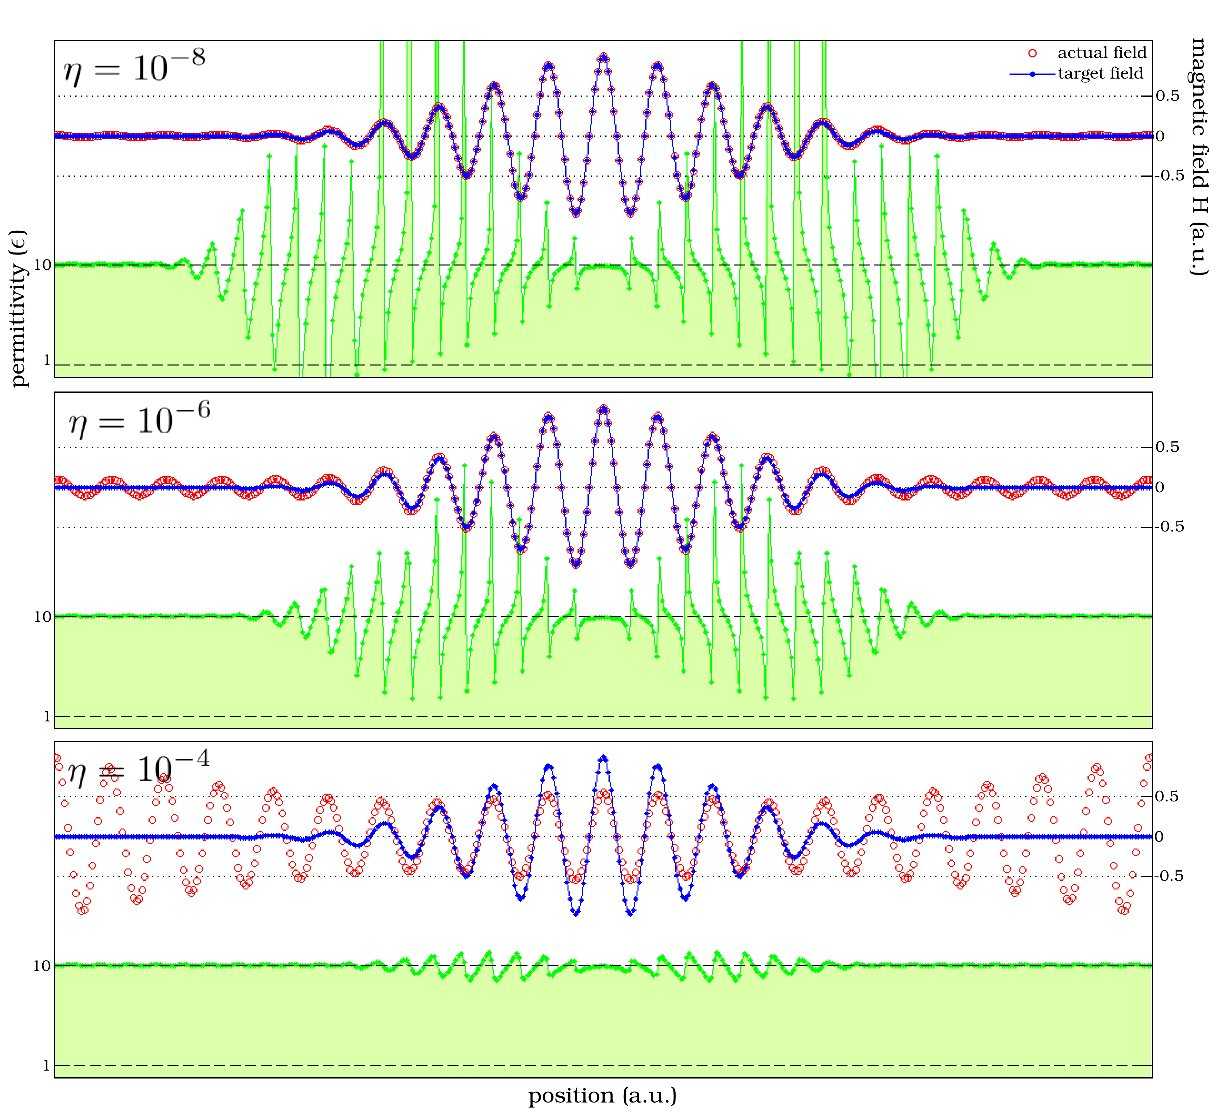
\includegraphics[width=\textwidth]{p1/regularized}
\caption{Inverse design of one-dimensional structures using the regularized least-squares method. The same target field is used as in Fig.~\ref{ls pic}, and the computation time remains below $1$ second. As the regularization parameter, $\eta$, is increased, $\epsilon$ is increasingly constrained to a chosen constant value of $10$. At the same time, the mismatch between target and actual fields increases markedly. This illustrates the apparent trade-off between producing reasonable structures and accurately reproducing a fixed target field.}
\label{regls pic}
\end{figure}
